%!TEX root = ../Main.tex

\section{Elements}

\subsection{Blocks}

\begin{frame}{Generic, Alert and Example blocks}
	% Generic block
	\begin{block}{Generic Block}
		Use this block to present important but non-urgent information. \cite{donnelly1997}
	\end{block}

	If you want to alert something, \alert{just do it}.
	% Alert block
	\begin{alertblock}{Alert Block}
		Use this alert block to highlight critical information or warnings that need immediate attention. \cite{chen2012}
	\end{alertblock}

	% Example block
	\begin{exampleblock}{Example Block}
		Use this block to provide examples or case studies. \cite{bredillet2018}
	\end{exampleblock}
\end{frame}

\begin{frame}{Theorem, Definition and Proof blocks}
	% Theorem block
	\begin{theorem}
		Use this block to present a formal statement that can be proven true. \cite{basl2002}
	\end{theorem}

	% Definition block
	\begin{definition}
		Use this block to define a term or concept clearly and precisely. \cite{bach2017}
	\end{definition}

	% Proof block
	\begin{proof}
		Use this block to provide the logical reasoning and steps needed to prove a theorem or proposition.
	\end{proof}
\end{frame}

\begin{frame}{Lemma and Corollary blocks}
	% Lemma block
	\begin{lemma}
		Use this block to present a lemma, which is a supporting statement or an intermediate result used to prove a larger theorem.
	\end{lemma}

	% Corollary block
	\begin{corollary}
		Use this block to present a corollary, which is a result that follows directly from a theorem or lemma.
	\end{corollary}
\end{frame}

\subsection{List Environments}

\begin{frame}{Unordered/Order List}
	\begin{columns}
		\begin{column}{0.5\textwidth}
			This is an unordered list:
			\begin{itemize}
				\item Item
				\item Item
				\item Item
			\end{itemize}
		\end{column}

		\begin{column}{0.5\textwidth}
			This is an ordered list:
			\begin{enumerate}
				\item Item
				\item Item
				\item Item
			\end{enumerate}
		\end{column}
	\end{columns}
\end{frame}

\begin{frame}{List With Item Labels}
	\begin{description}
		\item[Label] Some text
		\item[Label] Some text
		\item[Label] Some text
	\end{description}
\end{frame}

\subsection{Illustrations}

\begin{frame}{Figures}
	\begin{figure}[ht]
		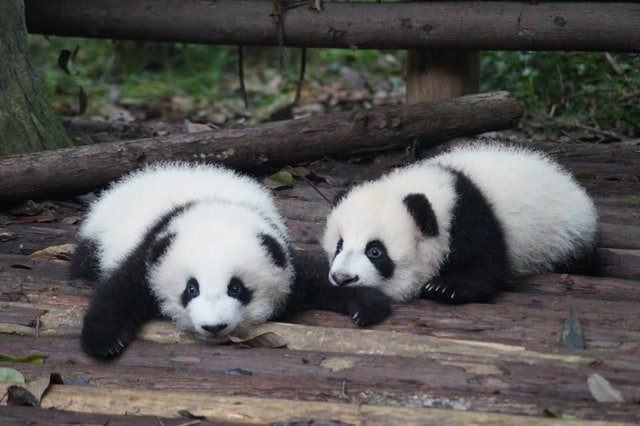
\includegraphics[width = 0.5\textwidth]{04-figures/panda-cubs.jpg}
		\caption{(\href{https://unsplash.com/photos/4EajIuUxgAQ}{Photo} by \href{https://unsplash.com/@millerthachiller}{Pascal M\"{u}ller} on \href{https://unsplash.com/}{Unsplash})}
	\end{figure}
\end{frame}

\begin{frame}{Tables}
	\begin{table}[ht]
		\centering
		%!TEX root = ../Main.tex

\begin{tabular}{c || cccc}
	\textbf{Employee ID \(ID_i\) (Key)} & \(ID_1\) & \(ID_2\) & \(\dots\) & \(ID_{\kappa}\) \\
	\hline
	\textbf{Employee Name \(Name_i\) (Value)} & John & Maria & \(\dots\) & \(Name_{\kappa}\) \\
\end{tabular}

		\caption{Table 1}
	\end{table}

	\begin{table}[ht]
		\centering
		%!TEX root = ../Main.tex

\begin{tabular}{||c c c c||}
	\hline
	Column 1 & Column 2 & Column 3 & Column 4 \\
	\hline\hline
	Value 1, 1 & Value 1, 2 & Value 1, 3 & Value 1, 4 \\
	\hline
	Value 2, 1 & Value 2, 2 & Value 2, 3 & Value 2, 4 \\
	\hline
	Value 3, 1 & Value 3, 2 & Value 3, 3 & Value 3, 4 \\
	\hline
	Value 4, 1 & Value 4, 2 & Value 4, 3 & Value 4, 4 \\
	\hline
	Value 5, 1 & Value 5, 2 & Value 5, 3 & Value 5, 4 \\
	\hline
\end{tabular}

		\caption{Table 2}
	\end{table}
\end{frame}